\documentclass[a4paper,11pt]{article}

\usepackage[utf8]{inputenc}
\usepackage[swedish]{babel}
\usepackage[top=1in,bottom=1in,left=1in,right=1in,headsep=.5in]{geometry}
\usepackage{hyperref}
\usepackage{graphicx}

\usepackage{array}
\newcolumntype{L}[1]{>{\raggedright\let\newline\\\arraybackslash\hspace{0pt}}m{#1}}
\newcolumntype{C}[1]{>{\centering\let\newline\\\arraybackslash\hspace{0pt}}m{#1}}
\newcolumntype{R}[1]{>{\raggedleft\let\newline\\\arraybackslash\hspace{0pt}}m{#1}}

\usepackage[yyyymmdd,hhmmss]{datetime}
\renewcommand{\dateseparator}{-}

\usepackage{mathptmx}    %Times Roman font
\usepackage{helvet}    %Helvetica, served as a model for arial
\usepackage{anyfontsize}

\usepackage[tocgraduated]{tocstyle}
\usetocstyle{allwithdot}

\usepackage[titletoc,title]{appendix}

\usepackage{fancyhdr}
\fancypagestyle{intro}{
    \fancyhf{}
    \fancyhead[C]{\LIPSprojekttitel}
    \fancyhead[R]{\today} 
    \fancyfoot[L]{\LIPSkursnamn \\ \LIPSdokumenttyp}
    \fancyfoot[C]{\phantom{text}\roman{page}}
    \fancyfoot[R]{\LIPSprojektgrupp \\ \LIPSgruppepost} 
    \renewcommand{\headrulewidth}{0.4pt}
    \renewcommand{\footrulewidth}{0.4pt}}
\fancypagestyle{content}{
    \fancyhf{}
    \fancyhead[C]{\LIPSprojekttitel}
    \fancyhead[R]{\today} 
    \fancyfoot[L]{\LIPSkursnamn \\ \LIPSdokumenttyp}
    \fancyfoot[C]{\phantom{text}\thepage}
    \fancyfoot[R]{\LIPSprojektgrupp \\ \LIPSgruppepost} 
    \renewcommand{\headrulewidth}{0.4pt}
    \renewcommand{\footrulewidth}{0.4pt}}

\usepackage{titlesec}
\titleformat{\section}
    {\normalfont\sffamily\Large\bfseries}
    {\thesection}{1em}{}
\titleformat{\subsection}
    {\normalfont\sffamily\Large\bfseries}
    {\thesubsection}{1em}{}
\titleformat{\subsubsection}
    {\normalfont\sffamily\Large\bfseries}
    {\thesubsubsection}{1em}{}

\newcommand{\LIPSartaltermin}{2016/HT}
\newcommand{\LIPSkursnamn}{TSEA29}
\newcommand{\LIPSprojekttitel}{Kartrobot}
\newcommand{\LIPSprojektgrupp}{Grupp 1}
\newcommand{\LIPSgruppepost}{\href{mailto:kmm_2016_grupp1@liuonline.onmicrosoft.com}{{\small kmm\_2016\_grupp1@liuonline.onmicrosoft.com}}}
\newcommand{\LIPSgrupphemsida}{}
\newcommand{\LIPSkund}{ISY, Linköpings universitet, 581\,83 Linköping}
\newcommand{\LIPSkundkontakt}{Mattias Krysander, 013-282198, matkr@isy.liu.se}
\newcommand{\LIPSkursansvarig}{Tomas Svensson, 013-281368, Tomas.Svensson@liu.se}
\newcommand{\LIPShandledare}{}
\newcommand{\LIPSdokumenttyp}{Kravspecifikation}
\newcommand{\LIPSredaktor}{Felix Härnström}
\newcommand{\LIPSversion}{0.1}
\newcommand{\LIPSgranskare}{}
\newcommand{\LIPSgranskatdatum}{}
\newcommand{\LIPSgodkannare}{}
\newcommand{\LIPSgodkantdatum}{}

\newcommand{\LIPStitelsida}{
\vspace*{200pt}
\renewcommand{\familydefault}{\sfdefault}	%Sans-serif
\normalfont
\begin{center}
{\fontsize{18}{22}\selectfont \textbf{\MakeUppercase{\LIPSdokumenttyp}}}
\end{center}
\begin{center}
{\fontsize{12}{14}\selectfont \LIPSredaktor \\[8pt] Version \LIPSversion}
\end{center}
\vspace*{220pt}
\begin{center}
{\fontsize{12}{14}\selectfont Status}
\end{center}
\begin{center}
\setlength\extrarowheight{2pt}
\begin{tabular}{| L{100pt} | L{100pt} | L{100pt} |}
\hline 
Granskad & \LIPSgranskare & \LIPSgranskatdatum \\
\hline 
Godkänd & \LIPSgodkannare & \LIPSgodkantdatum \\ 
\hline 
\end{tabular} 
\end{center}
\renewcommand{\familydefault}{\rmdefault}	%Back to serifs
\normalfont
}


\newenvironment{LIPSprojektidentitet}{%
\vspace*{200pt}
\renewcommand{\familydefault}{\sfdefault}	%Sans-serif
\normalfont
\begin{center}
{\fontsize{16}{19}\selectfont \textbf{PROJEKTIDENTITET}}
\end{center}
\renewcommand{\familydefault}{\rmdefault}	%Back to serifs
\normalfont
\begin{center}
\LIPSartaltermin, \LIPSprojektgrupp \\ Linköpings tekniska högskola, ISY
\end{center}
\renewcommand{\familydefault}{\sfdefault}	%Sans-serif
\normalfont
\vspace*{10pt}
\begin{center}
\setlength\extrarowheight{2pt}
\begin{tabular}{| L{100pt} | L{150pt} | L{150pt} |}
\hline
\textbf{Namn} & \textbf{Ansvar} & \textbf{E-post} \\
}%
{%
\hline
\end{tabular} 
\end{center}
\renewcommand{\familydefault}{\rmdefault}	%Back to serifs
\normalfont
\begin{center}
\textbf{E-postlista för hela gruppen:} \LIPSgruppepost \\
\textbf{Hemsida:} \LIPSgrupphemsida \\
\vspace*{15pt}
\textbf{Kund:} \LIPSkund \\
\textbf{Kontaktperson hos kund:} \LIPSkundkontakt \\
\vspace*{15pt}
\textbf{Kursansvarig:} \LIPSkursansvarig \\
\textbf{Handledare:} \LIPShandledare \\
\end{center}
}
\newcommand{\LIPSgruppmedlem}[3]{\hline {#1} & {#2} & \href{mailto:{#3}}{{#3}} \\}

\newenvironment{LIPSdokumenthistorik}{%
\vspace*{100pt}
\renewcommand{\familydefault}{\sfdefault}	%Sans-serif
\normalfont
\begin{center}
{\fontsize{14}{17}\selectfont \textbf{Dokumenthistorik}}
\end{center}
\begin{center}
\setlength\extrarowheight{2pt}
\begin{tabular}{| L{50pt} | L{60pt} | L{150pt} | L{60pt} | L{55pt} |}
\hline
\textbf{Version} & \textbf{Datum} & \textbf{Utförda förändringar} & \textbf{Utförda av} & \textbf{Granskad} \\
}%
{%
\hline
\end{tabular} 
\end{center}
\renewcommand{\familydefault}{\rmdefault}	%Back to serifs
\normalfont
}
\newcommand{\LIPSversionsinfo}[5]{\hline {#1} & {#2} & {#3} & {#4} & {#5} \\}

\newcounter{LIPSkravnummer}
\newcounter{LIPSunderkravnummer}[LIPSkravnummer]
\newenvironment{LIPSkravlista}{%
\renewcommand{\familydefault}{\sfdefault}	%Sans-serif
\normalfont
 \setlength\extrarowheight{2pt}
  \begin{tabular}{| L{30pt } | L{60pt} | L{250pt} | L{50pt} |}
    }%
  {%
    \hline
  \end{tabular}
\renewcommand{\familydefault}{\rmdefault}	%Back to serifs
\normalfont
}
\newcommand{\LIPSkrav}[3]{\hline\stepcounter{LIPSkravnummer}\textbf{\arabic{LIPSkravnummer}} & \textbf{{#1}} & {#2} & \textbf{{#3}} \\}

\newcommand{\LIPSkravDemo}[3]{\hline\textbf{X} & \textbf{{#1}} & {#2} & \textbf{{#3}} \\}

\newcommand{\LIPSunderkrav}[3]{\hline\stepcounter{LIPSunderkravnummer}\textbf{\arabic{LIPSkravnummer}\Alph{LIPSunderkravnummer}} & \textbf{{#1}} & {#2} & \textbf{{#3}} \\}


\newenvironment{LIPSleveranslista}{
\renewcommand{\familydefault}{\sfdefault}	%Sans-serif
\normalfont
	\setlength\extrarowheight{2pt}
	\begin{tabular}{| L{25mm} | L{25mm} | L{55mm} | L{25mm} | L{5mm} |} 
	}
	{
		\hline
	\end{tabular}
\renewcommand{\familydefault}{\rmdefault}	%Back to serifs
\normalfont
}
\newcommand{\LIPSleverans}[4]{ \hline\stepcounter{LIPSkravnummer}\textbf{Krav nr \arabic{LIPSkravnummer}}&\textbf{{#1}}&{#2}&\textbf{{#3}}&\textbf{{#4}}\\}


\newenvironment{LIPSdokumentlista}{%
	\renewcommand{\familydefault}{\sfdefault}	%Sans-serif
	\normalfont
	\setlength\extrarowheight{2pt}
	\begin{tabular}{| L{40mm} | L{13mm} | L{50mm} | L{19mm} | L{14mm} |} 
		
		\hline
		\textbf{Dokument} & \textbf{Språk} & \textbf{Syfte/Innehåll} & \textbf{Målgrupp} & \textbf{Format} \\
	}%
	{%
		\hline
	\end{tabular}
	\renewcommand{\familydefault}{\rmdefault}	%Back to serifs
	\normalfont
}
\newcommand{\LIPSdokument}[5]{\hline {#1} & {#2} & {#3} & {#4} & {#5}\\}

\begin{document}
\pagestyle{intro}
\LIPStitelsida
\clearpage
\begin{LIPSprojektidentitet}
    \LIPSgruppmedlem{Hannes Haglund}{}{hanha265@student.liu.se}
    \LIPSgruppmedlem{Felix Härnström}{Projektledare (PL)}{felha423@student.liu.se}
    \LIPSgruppmedlem{Jani Jokinen}{}{janjo273@student.liu.se}
    \LIPSgruppmedlem{Silas Lenz}{}{sille914@student.liu.se}
    \LIPSgruppmedlem{Daniel Månsson}{}{danma344@student.liu.se}
    \LIPSgruppmedlem{Emil Norberg}{Dokumentansvarig (DOK)}{emino969@student.liu.se}
\end{LIPSprojektidentitet}
\clearpage
\renewcommand{\familydefault}{\sfdefault}	%Sans-serif
\normalfont
\tableofcontents
\renewcommand{\familydefault}{\rmdefault}	%Back to serifs
\normalfont
\clearpage
\begin{LIPSdokumenthistorik}
    \LIPSversionsinfo{0.1}{2016-09-05}{Första utkastet}{FH}{FH}
\end{LIPSdokumenthistorik}
\clearpage
\setcounter{page}{1}
\pagestyle{content}
\section{Inledning}
\begin{figure}[h!]
    \makebox[\textwidth][c]{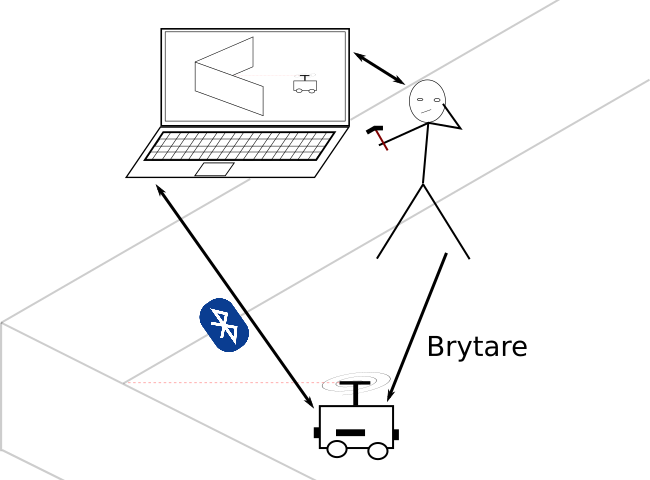
\includegraphics[width=1\textwidth]{overview.png}}
    \caption{Systemet i dess omgivning}
\end{figure}


I detta dokument kommer kravlistor formateras enligt figur \ref{fig:lipskrav_exempel}.
\begin{figure}[h!]
\begin{LIPSkravlista}
    \LIPSkravDemo{Förändring}{Kravtext för krav X}{Prioritet}
\end{LIPSkravlista}
\caption{Formatering för kravlista.}
\label{fig:lipskrav_exempel}
\end{figure}

Kravnummer i första kolumnen är formaterade löpande genom hela dokumentet. Andra kolumnen anger om det är ett originalkrav eller om kravet har reviderats. Den tredje kolumnen beskrivet kravet i text. Den fjärde kolumnen beskrivet kravets prioritet. Kravnivåerna är som följande:
\begin{itemize}
    \item Prioritetsnivå 1 – Kravet ska uppfyllas
    \item Prioritetsnivå 2 – Kravet ska uppfyllas om tid finns
    \item Prioritetsnivå 3 – Kravet ska uppfyllas efter att alla krav med nivå 2 uppfyllts 
\end{itemize}
\subsection{Parter}
Beställare: Mattias Krysander \\
Leverantör: \LIPSprojektgrupp \\
Handledare: xxx 

\subsection{Syfte och mål}
Att leverera en kartrobot som kan styras manuellt via Blåtand, samt autonomt kan navigera en bana, uppbyggd enligt bilaga \ref{sec:courseSpecification}, och samtidigt rita upp en karta över området.  
\subsection{Användning}
Roboten ska ha två lägen, ett för manuell fjärrstyrning, och ett autonomt läge. Man ska kunna växla mellan dessa lägen med en brytare på roboten. Det ska även finnas en startknapp på roboten. 
\subsubsection{Manuell styrning}
Vid manuell styrning så ska roboten reagera på följande kommandon som skickas via Blåtand: fram, fram vänster, fram höger, back, stopp, rotera vänster, rotera höger. 
\subsubsection{Autonom styrning}
I det autonoma läget ska roboten utforska en bana som är uppbyggd enligt bilaga \ref{sec:courseSpecification}. Den ska skicka data till en ansluten dator, som ritar upp en karta över området. Efter kartläggningen ska roboten returnera till startområdet. 
\subsection{Bakgrundsinformation}
\subsection{Definitioner}


\section{Översikt av systemet}

\subsection{Grov beskrivning av produkten}
Vår produkt är en robot som kan navigera genom en 6$ \times $6 m bana och kartlägga hur banan ser ut. Roboten ska ha två olika lägen; ett då den styrs med hjälp av Blåtand, ett annat då den är självkörande och kartlägger banan själv. Roboten ska även oavsett läge alltid skicka information angående sin status dvs data från sensorer, robotens läge etc. 

\subsection{Produktkomponenter}
Kartrobot med mjukvara till roboten samt för tillhörande dator, teknisk dokumentation, användarmanual, demonstration och en efterstudie. 

\subsection{Beroenden till andra system }
Beroenden till andra system 

\subsection{Ingående delsystem}
De moduler som ingår i konstruktionen är:
\begin{itemize}
    \item Sensorenhet (avläsning) 
    \item Styrenhet (styrning av motorer) 
    \item Kommunikations och kontrollenhet (Blåtand, beräkningar av rutt)  uppfyllts 
\end{itemize}

\subsection{Avgränsningar}
Behöver endast klara av banor utformade enligt bilaga \ref{sec:courseSpecification}. 
% TODO: vill vi ha Designfilosofi?

\subsection{Generella krav på hela systemet}
\begin{LIPSkravlista}
    \LIPSkrav{Original}{Roboten ska kunna bestämma avstånd till väggar.}{1}
    \LIPSkrav{Original}{Roboten ska kunna förflytta sig.}{1}
    \LIPSkrav{Original}{Roboten ska kunna styras manuellt av användaren via ett trådlöst medium (t.ex. Blåtand)}{1}
    \LIPSkrav{Original}{Roboten ska kunna styras autonomt.}{1}
    \LIPSkrav{Original}{Roboten ska undvika kollisioner i autonomt läge.}{1}
    \LIPSkrav{Original}{Roboten ska ha en fysisk brytare med vilken man kan välja mellan autonom och manuell styrning. }{1}
    \LIPSkrav{Original}{Roboten ska ha en fysisk brytare med vilken man startar den.}{1}
    \LIPSkrav{Original}{Roboten ska kunna kommunicera trådlöst med en bärbar dator.}{1}
    \LIPSkrav{Original}{Roboten ska skicka kartdata till en bärbar dator.}{1}
    \LIPSkrav{Original}{Roboten ska skicka styrdata till en bärbar dator.}{1}
    \LIPSkrav{Original}{Roboten ska skicka sensordata till en bärbar dator.}{1}
    \LIPSkrav{Original}{Roboten ska vara uppbyggd av utbytbara moduler.}{1}
    \LIPSkrav{Original}{I konstruktionen ska det ingå: kommunikationsmodul, styrenhet, samt sensorenhet.}{1}
    \LIPSkrav{Original}{Roboten ska återvända till ursprungspositionen efter kartläggning.}{1}
    \LIPSkrav{Original}{Roboten ska uppfylla kraven i bilaga \ref{sec:courseSpecification}.}{1}
    \LIPSkrav{Original}{Rummet som roboten kartlagt ska presenteras digitalt.}{1}
    \LIPSkrav{Original}{Den diagnostiska datan från roboten ska presenteras digitalt på den bärbara datorn.}{1}
    \LIPSkrav{Original}{Roboten ska kunna kartlägga ett rum som specificerat i bilaga \ref{sec:courseSpecification}.}{1}
\end{LIPSkravlista}

\newpage

\section{Delsystem 1 - Sensorenhet}
\begin{figure}[h!]
\centering
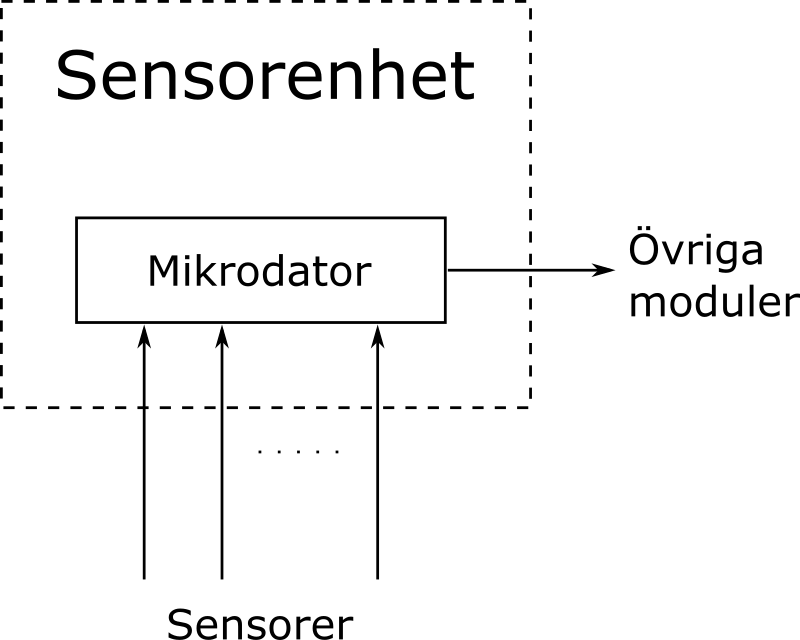
\includegraphics[scale=1]{sensorenhet.png}
\caption{Översiktligt blockschema för sensorenheten.}
\end{figure}

\subsection{Inledande beskrivning av delsystem 1}
Sensorenheten behandlar data från olika sensorer, för att sedan föra den vidare på ett läsligt format till styrenheten, delsystem 3.\\
\begin{LIPSkravlista}
    \LIPSkrav{Original}{Det ska sitta avståndssensorer på robotens sidor.}{1}
    \LIPSkrav{Original}{Det ska finnas nödstoppsfunktionalitet.}{2}
    \LIPSkrav{Original}{En sensor ska sitta på toppen av roboten för avläsning av rummet. Denna sensor ska rotera för att avläsa hela omgivningen}{1}
    \LIPSkrav{Original}{En sensor ska användas för kalibrering av graderna på den sensor som roterar för avläsning av rummet.}{2}
    \LIPSkrav{Original}{Roboten ska vara utrustad med ett gyro som håller reda på vilken riktning som roboten pekar.}{1}
\end{LIPSkravlista}

\subsection{Gränssnitt}
\begin{LIPSkravlista}
    \LIPSkrav{Original}{Sensoreneheten ska ta emot data från robotens sensorer}{1}
    \LIPSkrav{Original}{Sensorenheten ska, efter eventuell kalibrering, rapportera behandlad sensordata.}{1}
    \LIPSkrav{Original}{Sensorenheten ska indikera vilken sensor informationen kommer från.}{1}
    \LIPSkrav{Original}{Sensorenheten ska kunna skicka en nödstoppssignal.}{2}
\end{LIPSkravlista}

\subsection{Designkrav}
\begin{LIPSkravlista}
    \LIPSkrav{Original}{Sensorenheten ska arbeta med sex stycken avståndssensorer.}{1}
    \LIPSkrav{Original}{Sensorenheten ska vara skriven i C/C++.}{1}
    \LIPSkrav{Original}{Sensorenheten ska innehålla minst en processor.}{1}
\end{LIPSkravlista}

\subsection{Funktionella krav}
\begin{LIPSkravlista}
    \LIPSkrav{Original}{Enheten ska leverera data enligt givet protokoll.}{1}
    \LIPSkrav{Original}{Sensorenheten ska ta emot sensordata från sensorerna xxx}{1}
\end{LIPSkravlista}

\section{Delsystem 2 - Styrenhet}
\begin{figure}[h!]
\centering
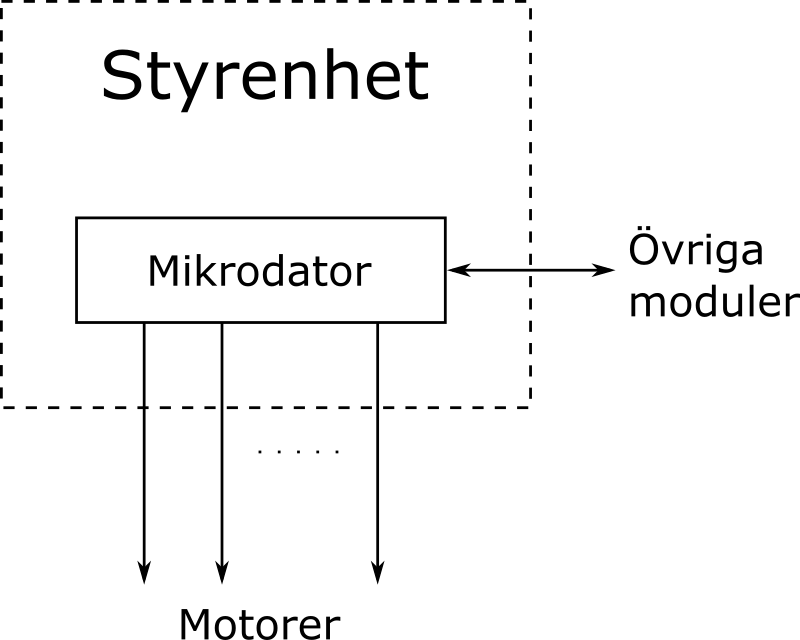
\includegraphics[scale=1]{styrenhet.png}
\caption{Översiktligt blockschema för styrenheten.}
\end{figure}


\subsection{Inledande beskrivning av delsystem 2}
Styrenheten är ansvarig för all logik och funktionalitet av robotens styrning. Styrenheten är länken mellan alla styrkommandon och motorerna, dvs att den ingående data måste följa ett givet protokoll. Den enda enhet som styrenhet kommunicerar med är kommunikations enheten.
% TODO: Ingen kravlista?

\subsection{Gränssnitt}
\begin{LIPSkravlista}
    \LIPSkrav{Original}{Styrenheten ska styra alla motorer i konstruktionen.}{1}
    \LIPSkrav{Original}{Enheten ska kunna ta emot styrinstruktioner på ett väldefinierat format.}{1}
    \LIPSkrav{Original}{Styrenheten ska kunna rapportera styrdata.}{1}
    \LIPSkrav{Original}{Sensorenheten ska kunna ta emot en nödstoppssignal.}{2}
\end{LIPSkravlista}

\subsection{Designkrav}
\begin{LIPSkravlista}
    \LIPSkrav{Original}{Styrenheten ska arbeta med servomotorerna xxx}{1}
    \LIPSkrav{Original}{Styrenheten ska vara skriven i C/C++.}{1}
    \LIPSkrav{Original}{Styrenheten ska innehålla minst en processor.}{1}
\end{LIPSkravlista}

\subsection{Funktionella krav}
\begin{LIPSkravlista}
    \LIPSkrav{Original}{Enheten ska ta emot data enligt givet protokoll.}{1}
    \LIPSkrav{Original}{Enheten ska styra servomotorerna xxx}{1}
    \LIPSkrav{Original}{Styrenheten ska kunna översätta högnivåinstruktioner som exempelvis ''hastighet n rakt fram'' och ''sväng 10 grader åt höger'' till motorsignaler.}{2}
\end{LIPSkravlista}

\section{Delsystem 3 - Kommunikations och kontrollenhet }
\begin{figure}[h!]
    \centering
    
\includegraphics[scale=1]{brain.png} %TODO Ska blåtandsenheten ritas inuti enkortsdatorn?
    \caption{Översiktligt blockschema för kommunikations och kontrollenheten.}
\end{figure}


\subsection{Inledande beskrivning av delsystem 3}
Kommunikationsenheten kommunicerar med modulerna på själva roboten, och med PC:n. I samma hårdvarumodul ingår också kontrollenheten, som gör beräkningar relaterat till det autonoma läget.

\subsection{Gränssnitt}
\begin{LIPSkravlista}
    \LIPSkrav{Original}{Ska ta emot data sensordata.}{1}
    \LIPSkrav{Original}{Ska kunna skicka motorinstruktioner.}{1}
    \LIPSkrav{Original}{Enheten ska kunna skicka motorinstruktioner på hög nivå, t.ex. ''hastighet n rakt fram'' och ''sväng 10 grader åt höger''. }{2}
    \LIPSkrav{Original}{Enheten ska ta emot styrdata efter utfört högnivåkommando (se föregående krav).}{2}
    \LIPSkrav{Original}{Kommunikationsenheten ska ta emot kommandon från PC-mjukvaran via Blåtand.}{1}
    \LIPSkrav{Original}{Enheten ska skicka sensor- och motordata till PC:n via Blåtand.}{1}
\end{LIPSkravlista}

\subsection{Designkrav}
\begin{LIPSkravlista}
    \LIPSkrav{Original}{arg2}{1}
    \LIPSkrav{Original}{arg2}{1}
    \LIPSkrav{Original}{arg2}{1}
    \LIPSkrav{Original}{arg2}{1}
    \LIPSkrav{Original}{arg2}{1}
    \LIPSkrav{Original}{arg2}{1}
    \LIPSkrav{Original}{arg2}{1}
    \LIPSkrav{Original}{arg2}{1}
\end{LIPSkravlista}

\subsection{Funktionella krav}
\begin{LIPSkravlista}
    \LIPSkrav{Original}{Kontrollenheten ska kunna konstruera en mjukvarurepresentation av det fysiska rummet.}{1}
    \LIPSkrav{Original}{Kontrollenheten ska kunna bestämma en kollisionsfri färdväg genom dess mjukvarurepresentation av det fysiska rummet.}{1}
    \LIPSkrav{Original}{Kontrollenheten ska bestämma lämpliga styrinstruktioner för att navigera genom det fysiska rummet utan kollisioner med väggar.}{1}
    \LIPSkrav{Original}{Då delar av rummet är outforskade så ska kontrollenheten kunna bestämma vägar till punkter som tillåter roboten att skanna outforskade delar av rummet.}{1}
    \LIPSkrav{Original}{Då delar av rummet är outforskat ska kontrollenheten skicka styrinstruktioner för att navigera till punkter som tillåter roboten att skanna outforskade delar av rummet.}{1}
    \LIPSkrav{Original}{Då roboten stannar på en punkt som tillåter den att skanna outforskade delar av rummet ska den kunna göra detta, och uppdatera sin mjukvarurepresenation av det fysiska rummet.}{1}
    \LIPSkrav{Original}{Då roboten inte längre kan nå outforskade delar av det fysiska rummet så ska kontrollenheten skicka instruktioner som resulterar i att roboten återvänder till sin startpunkt.}{1}
\end{LIPSkravlista}


\section{Delsystem 4 - Mjukvara på PC}
\begin{figure}[h!]
    \centering
    
\includegraphics[scale=1]{PC.png} 
    \caption{Översiktligt blockschema över PC-mjukvaran}
\end{figure}

\subsection{Inledande beskrivning av delsystem 4}
För att den manuella navigeringen ska fungera måste den dator som skickar kommandon över Blåtand ha mjukvara som stödjer detta. Mjukvaran ska inte bara förbereda dina kommandon för ett lämpligt protokoll men även sända kommandot över Blåtand. 

\subsection{Gränssnitt}
\begin{LIPSkravlista}
    \LIPSkrav{Original}{Mjukvaran ska skicka kommandon för navigering som roboten kan avläsa och utföra.}{1}
    \LIPSkrav{Original}{Kommandon för navigering ska skickas över Blåtand.}{1}
    \LIPSkrav{Original}{Sensorernas värden och robotens status ska skickas tas emot över Blåtand och presenteras för användaren.}{1}
    \LIPSkrav{Original}{Den karta som är genererad av roboten ska kunna ritas ut i denna mjukvara.}{1}
\end{LIPSkravlista}

\subsection{Designkrav}
\begin{LIPSkravlista}
    \LIPSkrav{Original}{Mjukvaran ska kommunicera med roboten över Blåtand.}{1}
    \LIPSkrav{Original}{Datan för att hämta karta samt skicka kommandon sker över samma protokoll.}{2}
\end{LIPSkravlista}

\subsection{Funktionella krav}
\begin{LIPSkravlista}
    \LIPSkrav{Original}{Mjukvaran ska rita ut kartan som ett tydlig rutnät i storlek 17x17, där varje cell är antingen en vägg eller öppen yta och ska representera en 40x40 centimeters verklig yta.}{1}
    \LIPSkrav{Original}{Robotens och sensorernas status samt den hitintills genererade kartan presenteras uppdateras kontinuerligt i mjukvaran.}{2}
\end{LIPSkravlista}

\section{Prestandakrav}
\begin{LIPSkravlista}
    \LIPSkrav{Original}{Roboten ska kunna kartlägga ett rum som specificerat i bilaga \ref{sec:courseSpecification} på under 20 minuter}{1}
    \LIPSkrav{Original}{Roboten ska kunna skanna rummet medan den rör sig, det vill säga den behöver inte stanna för att söka efter väggar omkring sig.}{2}
\end{LIPSkravlista}


\section{Krav på vidareutveckling}


\section{Tillförlitlighet}


\section{Ekonomi}

\begin{LIPSkravlista}
    \LIPSkrav{Original}{Gruppen ska ha arbetat sammanlagt maximalt 960 timmar vid leverans.}{1}
\end{LIPSkravlista}

\section{Leveranskrav och delleveranser}
\begin{LIPSleveranslista}
    \LIPSleverans{Original}{Kravspecifikation}{2016-09-13}{1}
    \LIPSleverans{Original}{Första versionen av projektplan, tidplan och systemskiss}{2016-09-23}{1}
    \LIPSleverans{Original}{Slutgiltig version av projektplan, tidplan och systemskiss}{2016-09-29}{1}
    \LIPSleverans{Original}{Första versionen av designspecifikationen}{2016-11-01}{1}
    \LIPSleverans{Original}{Slutgiltig version av designspecifikation}{2016-11-04}{1}
    \LIPSleverans{Original}{Teknisk dokumentation och användarhandledning}{3 arbetsdagar före redovisning}{1}
    \LIPSleverans{Original}{Verifiering av kraven (BP5).}{Senast dagen innan redovisning}{1}
    \LIPSleverans{Original}{Redovisning och demonstration}{Vecka 51}{1}
    \LIPSleverans{Original}{Slutpresentation}{2016-12-19}{1}
    \LIPSleverans{Original}{Tävlingsdeltagande}{2016-12-20}{1}
    \LIPSleverans{Original}{Efterstudie samt inlämning av källkod}{2016-12-21}{1}
    \LIPSleverans{Original}{Tidrapporter}{31/10, 7/11, 14/11, 21/11, 28/11, 5/12, 12/12, 19/12}{1}
\end{LIPSleveranslista}

\section{Dokumentation}
\begin{LIPSdokumentlista}
    \LIPSdokument{Teknisk dokumentation}{SV}{Beskrivning av konstruktionen för framtida underhåll, felsökning och konstruktionsunderlag}{Ingenjörer}{PDF}
    \LIPSdokument{Användarhandledning}{SV}{Beskrivning av hur produkten installeras och används}{Användare}{Wiki}
\end{LIPSdokumentlista}

\clearpage

\begin{appendices}

%TODO Appendix A and B are not at their final version. Update them as the original document updates.
\section{Specifikation för bana och tävling}

\subsection{Banspecifikation} \label{sec:courseSpecification}

\begin{figure}[h!]
\centering
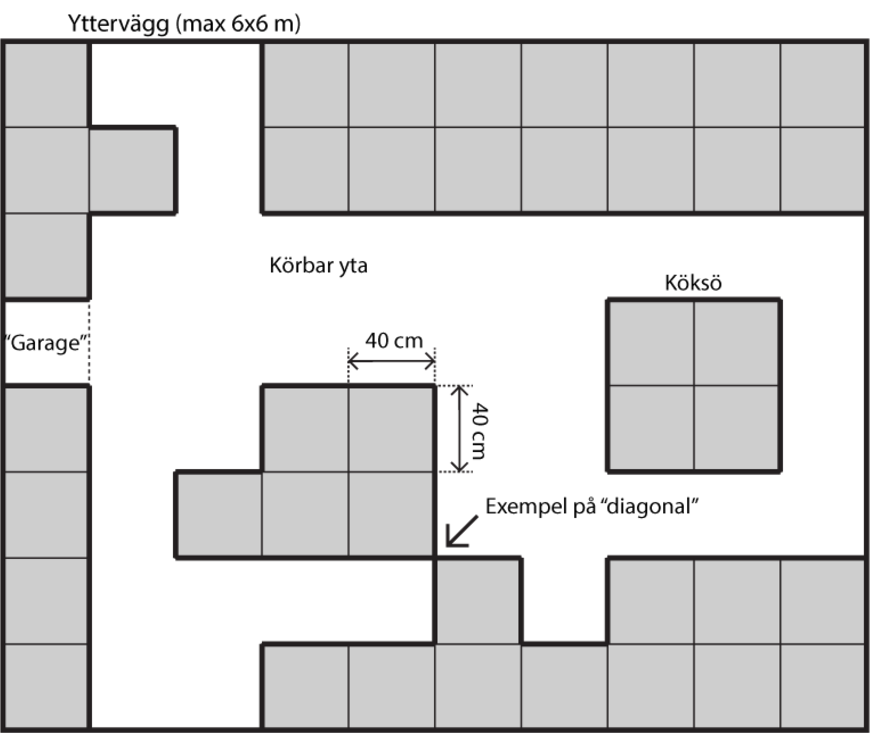
\includegraphics[scale=0.30]{banexempel.png}
\caption{Ett exempel på en tillåten bana.}
\end{figure}

\subsubsection{Enligt projektdirektiv}
\begin{itemize}
    \item Banan som roboten ska utforska är uppbyggd av kartongväggar, hädanefter kallat väggar, max 6x6 meter från vägg till vägg.
    \item Kartongväggarna skall ha längder som är multipler av 40 cm.
    \item Det skall ej vara möjligt att kartlägga kartongvärlden genom att endast följa en vägg.
    \item Alla hörn ska ha en vinkel av 90 grader.
    \item Exakt en köksö skall förekomma.
    \item Den sida på köksön som är närmast ytterväggen ska ha ett avstånd till ytterväggen på max 80 cm.
\end{itemize}

\subsubsection{Tillägg}
\begin{LIPSAppendixKravlista}
    \LIPSAppendixKrav{Original}{Startpunkten ska definieras som ett ''garage'': en ruta i rutnätet med väggar på tre sidor, 40x40 centimeter.}
    \LIPSAppendixKrav{Original}{Målet ska vara densamma som startpunkten.}
    \LIPSAppendixKrav{Original}{Roboten ska få starta och sluta roterad i valfri riktning.}
    \LIPSAppendixKrav{Original}{''Garaget'' ska vara placerat i ytterväggen (inte i köksön).}
    \LIPSAppendixKrav{Original}{Ytan av ''garaget'' ska inkluderas i de 6x6 meter som utgör banan.}
    \LIPSAppendixKrav{Original}{Alla kartongväggar ska vara delar i ''väggceller'' som upptar en avskärmad yta på 40x40 centimeter. Kartongväggar inuti oåtkomliga områden (ur robotens perspektiv) krävs ej.}
    \LIPSAppendixKrav{Original}{Köksöns väggceller ska ej vara förskjutna i rutnätet som bildas av rummets alla celler.}
    \LIPSAppendixKrav{Original}{''Diagonaler'' ska vara tillåtna, det vill säga väggceller som endast delar ett gemensamt hörn.}
    \LIPSAppendixKrav{Original}{Golvet ska utgöras av laminatgolv à LiU-standard.}
\end{LIPSAppendixKravlista}


\subsection{Tävlingsregler}

\subsubsection{Tävlingsupplägg}
\begin{LIPSAppendixKravlista}
    \LIPSAppendixKrav{Original}{Varje robot ska köra två heat.}
    \LIPSAppendixKrav{Original}{Det bästa av de två heaten ska räknas.}
    \LIPSAppendixKrav{Original}{Båda heaten ska köras på samma bana.}
    \LIPSAppendixKrav{Original}{Roboten ska autonomt köra sitt heat utan yttre påverkan från gruppens medlemmar.}
    \LIPSAppendixKrav{Original}{Mellan heaten ska grupperna få chans att laga sin robot vid uppenbara skador, men det ges ej möjlighet att förbättra roboten från dess utförande vid leverans, t.ex. förändra kod, förändra konfiguration eller bygga på fler komponenter.}
    \LIPSAppendixKrav{Original}{Tid tas under tävling, och klockan ska stoppas då roboten har läst in ett sammanhängande rum och återvänt till “Garaget”, mer precist då alla fyra hjulen befinner sig i den cellen. Ett sammanhängande rum ska definieras som en yta helt innesluten i väggar.}
    \LIPSAppendixKrav{Original}{Ett heat ska avslutas då klockan stoppas..}
    \LIPSAppendixKrav{Original}{Resultatet ska vara på formen av ett rutnät . Varje cell ska representera en 40x40 centimeter cell i tävlingsområdet, och ska antingen vara definierad som omsluten av väggar eller öppen.}
\end{LIPSAppendixKravlista}

\subsubsection{Diskvalifikation}
\begin{LIPSAppendixKravlista}
    \LIPSAppendixKrav{Original}{Om robotens höjd överstiger väggarnas höjd ska roboten diskvalificeras från det pågående heatet.}
    \LIPSAppendixKrav{Original}{Om roboten överskrider maxtiden XX minuter ska roboten diskvalificeras från det pågående heatet.}
    \LIPSAppendixKrav{Original}{Om gruppens system inte har visat en karta då roboten nått målet ska roboten diskvalificeras från det pågående heatet.}
    \LIPSAppendixKrav{Original}{Om en gruppmedlem intar banan eller vidrör en robot innan det pågående heatet är slut så ska gruppens robot diskvalificeras från det pågående heatet.}
\end{LIPSAppendixKravlista}

\subsubsection{Tidspålägg}
\begin{LIPSAppendixKravlista}
    \LIPSAppendixKrav{Original}{Tidspålägg fås därefter vid någon eller fler av följande händelser. Specificerade antal sekunder i tidspålägg bestäms av beställarna.}
    \LIPSAppendixKrav{Original}{Vidrörning av vägg ska ge ett tidspålägg på XX sekunder. Endast de vertikala bitarna av kartongväggarna ska räknas som en vägg.}
    \LIPSAppendixKrav{Original}{Utritning av felaktig karta. Tidspålägg ska ges per felaktigt ritat block, à XX sekunder. Vid fler än tre felaktiga block ska det istället för att ges tidspålägg per block ges ett enda tidspålägg på XX sekunder.}
\end{LIPSAppendixKravlista}


\end{appendices}


\end{document}
